
\section{Синтез $H_\infty$-оптимального управления}

\subsection{Расчёт оптимального регулятора}

Рассмотрим возмущённый линейный объект управления
\[
\dot{x}=Ax+Bu+B_f f
\]

Для варианта 23 заданы матрицы
\[
A=
\begin{pmatrix}
0&3\\
4&0
\end{pmatrix},
\qquad
B=
\begin{pmatrix}
0\\
2
\end{pmatrix},
\qquad
B_f=
\begin{pmatrix}
1\\
1
\end{pmatrix}
\qquad
Q=
\begin{pmatrix}
5&0\\
0&8
\end{pmatrix}
\]

Требуется построить $H_\infty$-оптимальный регулятор вида
\[
u=Kx
\]

Матрица усиления определяется выражением
\[
K=-B^TP
\]

где матрица $P$ является положительно полуопределённым
решением алгебраического уравнения Риккати
\[
A^TP+PA+Q-PBB^TP+
\gamma^{-2}PB_fB_f^TP=0
\]

Представим матрицу $P$ в симметричном виде
\[
P=
\begin{pmatrix}
p_{11}&p_{12}\\
p_{12}&p_{22}
\end{pmatrix}
\]

Вычислим слагаемые уравнения Риккати:
\[
A^TP+PA=
\begin{pmatrix}
8p_{12}&3p_{11}+4p_{22}\\
3p_{11}+4p_{22}&6p_{12}
\end{pmatrix}
\]

Поскольку
\[
BB^T=
\begin{pmatrix}
0&0\\
0&4
\end{pmatrix}
\]
получим
\[
PBB^TP=
4\begin{pmatrix}
p_{12}^2&p_{12}p_{22}\\
p_{12}p_{22}&p_{22}^2
\end{pmatrix}
\]

Аналогично
\[
B_fB_f^T=
\begin{pmatrix}
1&1\\
1&1
\end{pmatrix}
\]

\[
PB_fB_f^TP=
\begin{pmatrix}
(p_{11}+p_{12})^2&
(p_{11}+p_{12})(p_{12}+p_{22})\\
(p_{11}+p_{12})(p_{12}+p_{22})&
(p_{12}+p_{22})^2
\end{pmatrix}
\]

Подставляя полученные выражения в уравнение Риккати,
получаем систему трёх нелинейных уравнений
\[
\begin{cases}
8p_{12}+5-4p_{12}^2+
\gamma^{-2}(p_{11}+p_{12})^2=0\\[2mm]
3p_{11}+4p_{22}-4p_{12}p_{22}+
\gamma^{-2}(p_{11}+p_{12})(p_{12}+p_{22})=0\\[2mm]
6p_{12}+8-4p_{22}^2+
\gamma^{-2}(p_{12}+p_{22})^2=0
\end{cases}
\]

Для определения матрицы $P$ при заданном $\gamma$
данная система решается численно с использованием
алгебраического уравнения Риккати.

\subsection{Определение минимального значения $\gamma$}

Необходимо определить минимальное
значение $\gamma$, при котором существует положительно
полуопределённое стабилизирующее решение уравнения Риккати.

Для численного поиска использован метод деления отрезка
пополам на интервале
\[
\gamma\in[1,2]
\]

На каждой итерации решалось уравнение Риккати и проверялись
условия
\[
P\succeq0
\]

\[
\operatorname{Re}\lambda_i
\left(
A-BB^TP+\gamma^{-2}B_fB_f^TP
\right)<0
\]

Дополнительно контролировалась невязка уравнения Риккати.

После 40 итераций получено численное приближение
минимального допустимого значения:
\[
\gamma_{\min}\approx1{,}36381628
\]

Для дальнейших расчётов принято
\[
\gamma=\gamma_{\min}
\]

При найденном значении параметра получено решение
\[
P\approx10^4
\begin{pmatrix}
5{,}8772&3{,}4020\\
3{,}4020&1{,}9694
\end{pmatrix}
\]

В рамках численной проверки матрица $P$ удовлетворяет
условию положительной полуопределённости.

Матрица усиления регулятора определяется аналитически:
\[
\begin{aligned}
K&=-B^TP=-\begin{pmatrix}0&2\end{pmatrix}
\begin{pmatrix}
p_{11}&p_{12}\\
p_{12}&p_{22}
\end{pmatrix}=\begin{pmatrix}-2p_{12}&-2p_{22}\end{pmatrix}
\end{aligned}
\]

Подставляя найденные значения, получаем
\[
K\approx10^4
\begin{pmatrix}
-6{,}8041&-3{,}9388
\end{pmatrix}
\]

Таким образом, закон управления имеет вид
\[
u(t)=k_1x_1(t)+k_2x_2(t)
\]

где
\[
k_1\approx-6{,}8041\cdot10^4,
\qquad
k_2\approx-3{,}9388\cdot10^4
\]

\subsection{Исследование устойчивости замкнутой системы}

Подставим закон управления $u=Kx$ в уравнение объекта:
\[
\dot{x}=(A+BK)x+B_ff
\]

Матрица замкнутой системы имеет вид
\[
\begin{aligned}
A+BK
&=
\begin{pmatrix}
0&3\\
4&0
\end{pmatrix}
+
\begin{pmatrix}
0\\
2
\end{pmatrix}
\begin{pmatrix}
k_1&k_2
\end{pmatrix}=
\begin{pmatrix}
0&3\\
4+2k_1&2k_2
\end{pmatrix}
\end{aligned}
\]

Для исследования устойчивости определим
характеристический многочлен:
\[
\begin{aligned}
\det(\lambda I-(A+BK))
&=
\begin{vmatrix}
\lambda&-3\\
-(4+2k_1)&\lambda-2k_2
\end{vmatrix}=\lambda(\lambda-2k_2)-3(4+2k_1)\\
&=\lambda^2-2k_2\lambda-12-6k_1
\end{aligned}
\]

По критерию Гурвица для системы второго порядка
необходимо и достаточно выполнения условий
\[
\begin{cases}
-2k_2>0\\
-12-6k_1>0
\end{cases}
\]

Отсюда получаем область устойчивых значений
коэффициентов регулятора:
\[
\begin{cases}
k_1<-2\\
k_2<0
\end{cases}
\]

Найденные коэффициенты удовлетворяют обоим условиям.

Численно вычисленные собственные значения
матрицы замкнутой системы:
\[
\lambda_1\approx-5{,}18
\]

\[
\lambda_2\approx-7{,}877\cdot10^4
\]

Оба собственных значения отрицательны, следовательно,
замкнутая система является асимптотически устойчивой.

Большая разница между модулями собственных значений
указывает на наличие существенно различающихся
временных масштабов переходных процессов.

\subsection{Моделирование возмущённой системы}

Моделирование проведено при начальных условиях
\[
x(0)=
\begin{pmatrix}
1\\
0
\end{pmatrix}
\]

Внешнее возмущение задано функцией
\[
f(t)=10\sin(6t)+5\cos(2t)+4\cos(3t)+3\cos(8t)
\]

Решение уравнения замкнутой системы в общем виде
можно записать аналитически:
\[
x(t)=e^{(A+BK)t}x(0)+
\int_0^t e^{(A+BK)(t-\tau)}B_ff(\tau)\,d\tau
\]

Первое слагаемое описывает свободное движение системы,
а второе - вынужденное движение под действием возмущения.

Моделирование выполнено на интервале
\[
t\in[0,10]
\]

На рисунке~\ref{fig:task6_states} представлены
переменные состояния $x_1(t)$, $x_2(t)$ и управляющее
воздействие $u(t)$.

\begin{figure}[H]
    \centering
    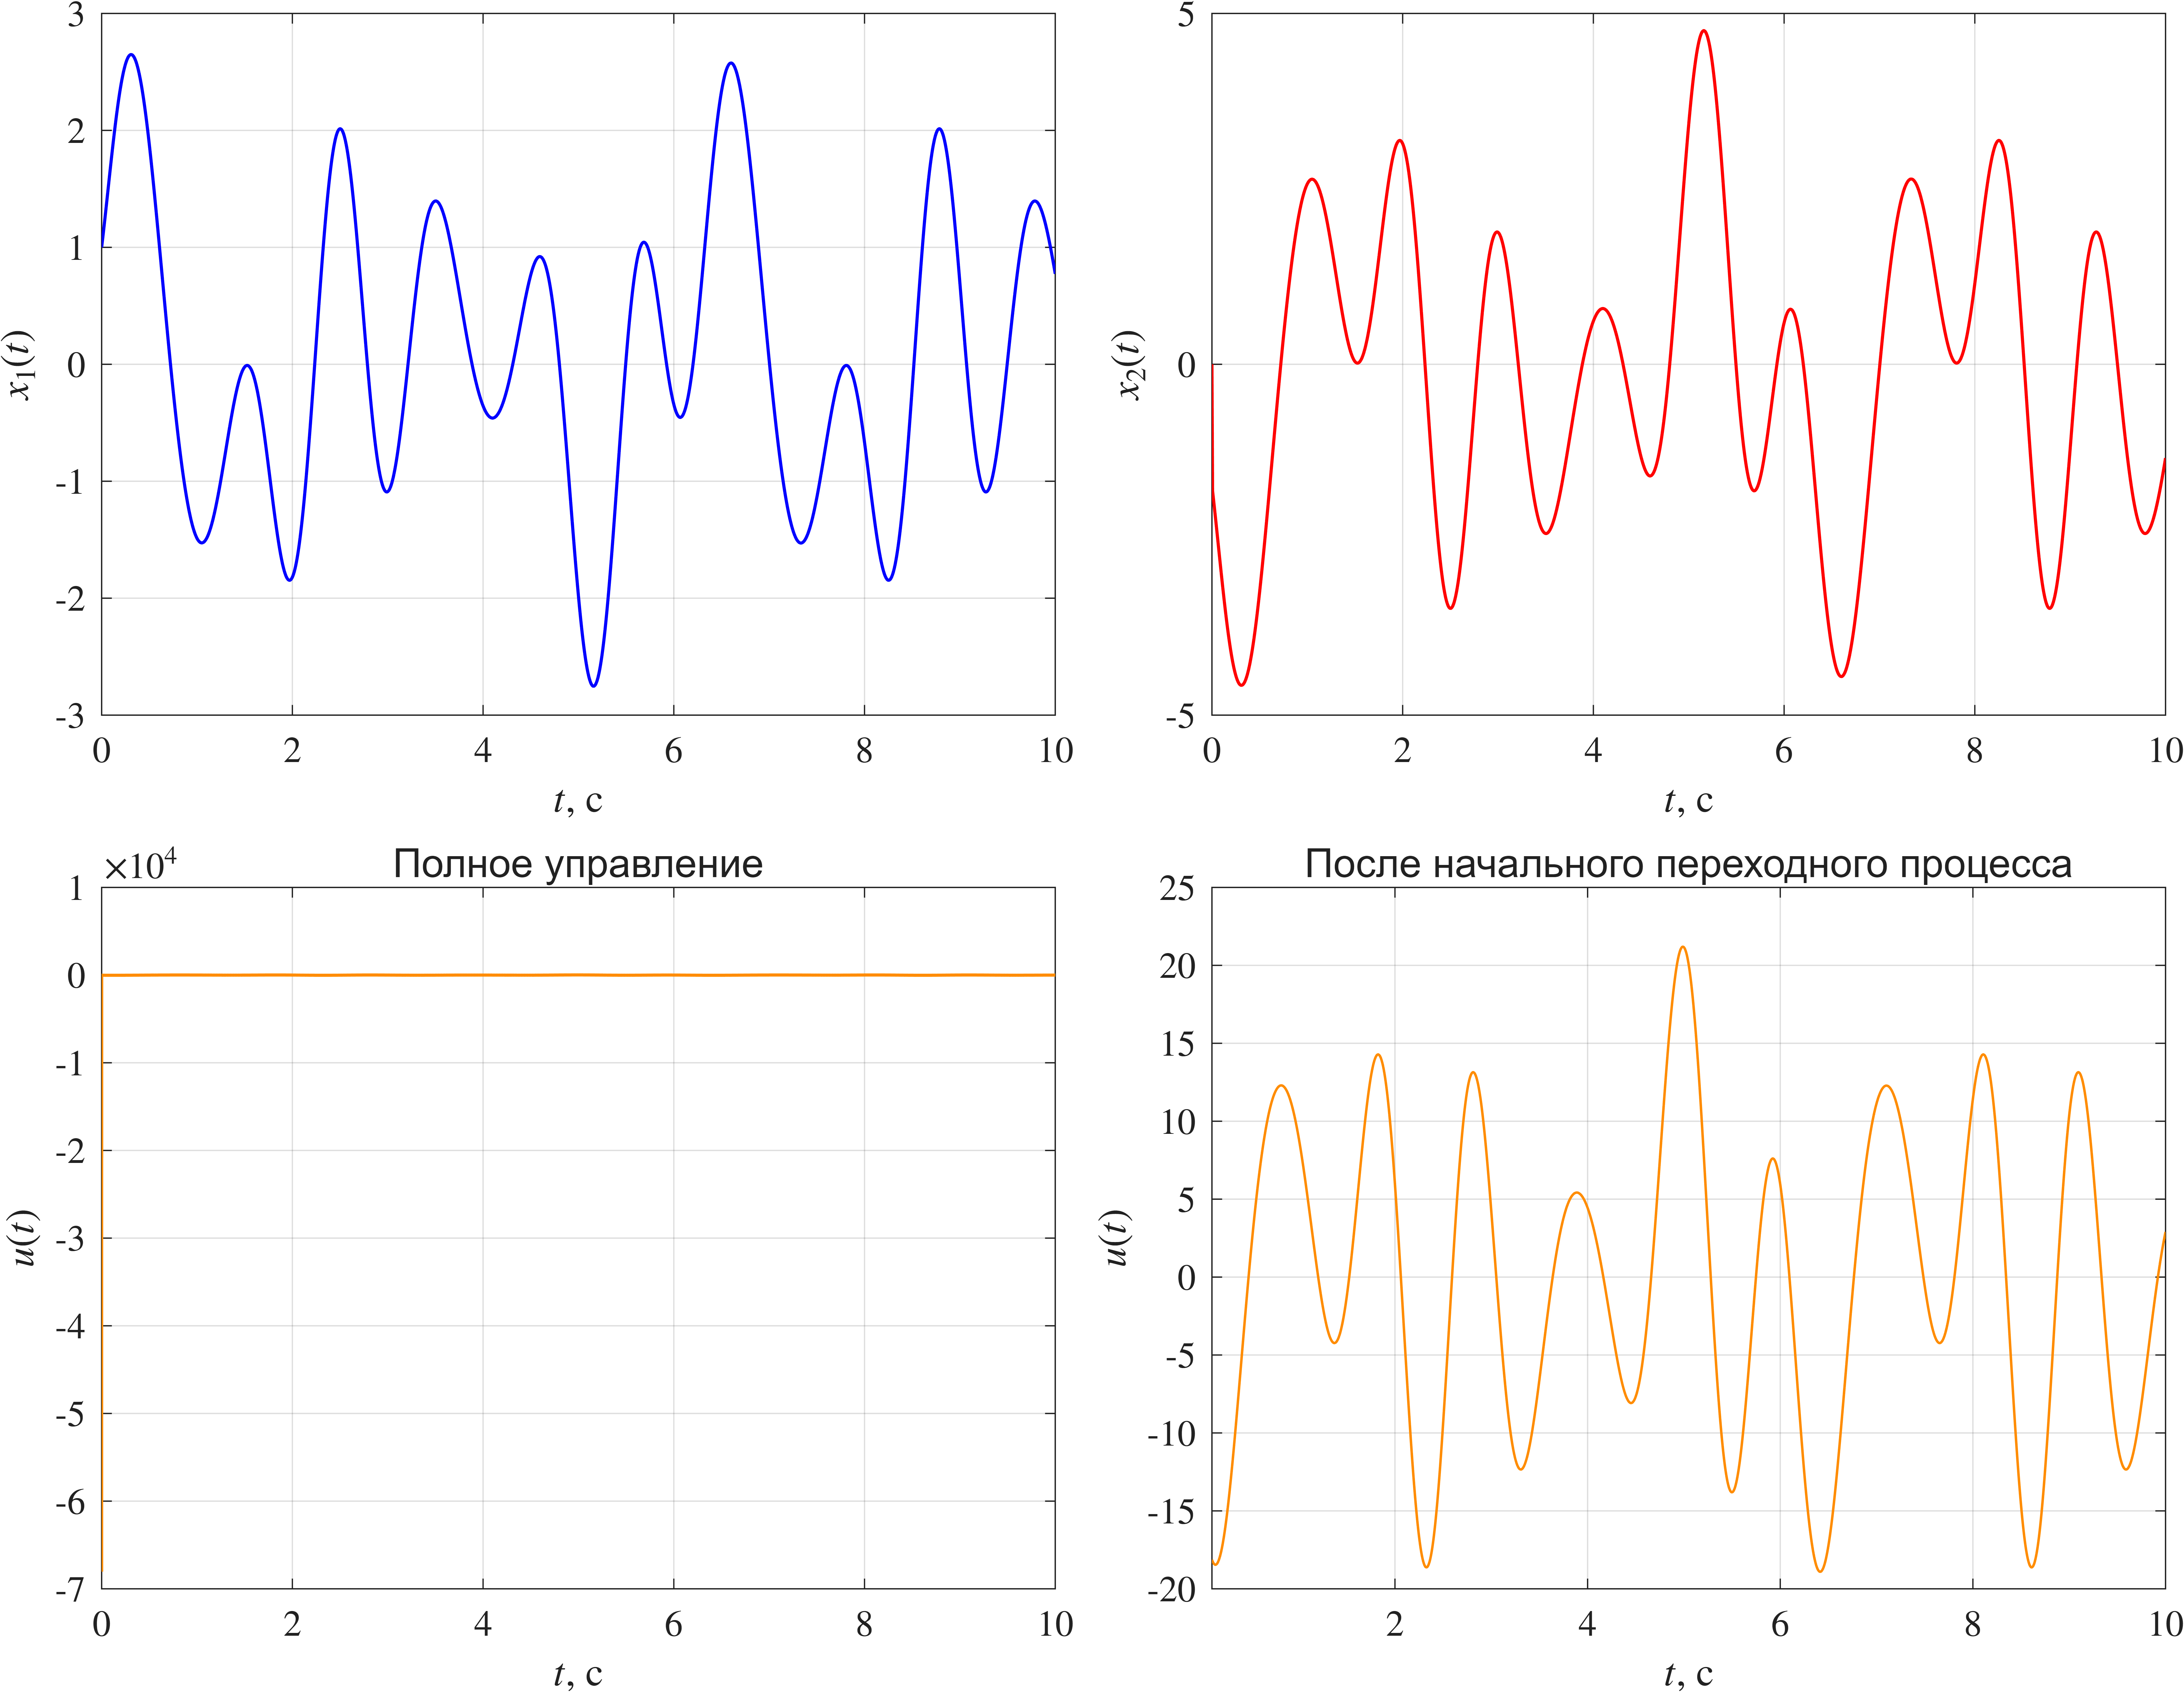
\includegraphics[width=0.95\textwidth]{images/task6_states.png}
    \caption{Переменные состояния и управляющее воздействие при $\gamma=\gamma_{\min}$}
    \label{fig:task6_states}
\end{figure}

Из результатов моделирования видно, что переменные
состояния совершают ограниченные колебания под действием
заданного периодического возмущения.

В начальный момент времени управление определяется
выражением
\[
u(0)=Kx(0)=k_1
\]

Следовательно,
\[
u(0)\approx-6{,}8041\cdot10^4
\]

Большой начальный выброс обусловлен высокими
коэффициентами усиления, полученными при предельном
значении $\gamma$.

После завершения быстрого начального переходного
процесса управление изменяется плавно и компенсирует
периодическое возмущение.

На графике полного управления начальный выброс
приводит к значительному увеличению масштаба оси ординат.
Поэтому дополнительно приведён график управления
на интервале $t\in[0{,}1;10]$~с.

Состояния системы остаются ограниченными, что согласуется
с результатами анализа устойчивости.

\subsection{Определение $H_\infty$-норм передаточных функций}

Для оценки влияния внешнего возмущения на отдельные
переменные состояния рассмотрим передаточные функции
\[
H_1(s)=C_1(sI-(A+BK))^{-1}B_f
\]

\[
H_2(s)=C_2(sI-(A+BK))^{-1}B_f
\]

где
\[
C_1=\begin{pmatrix}1&0\end{pmatrix},
\qquad
C_2=\begin{pmatrix}0&1\end{pmatrix}
\]

Найдём матрицу
\[
sI-(A+BK)=
\begin{pmatrix}
s&-3\\
-(4+2k_1)&s-2k_2
\end{pmatrix}
\]

Её определитель равен
\[
D(s)=s^2-2k_2s-12-6k_1
\]

По формуле обращения матрицы второго порядка:
\[
(sI-(A+BK))^{-1}
=
\frac{1}{D(s)}
\begin{pmatrix}
s-2k_2&3\\
4+2k_1&s
\end{pmatrix}
\]

Учитывая $B_f=(1,1)^T$, получаем
\[
(sI-(A+BK))^{-1}B_f
=
\frac{1}{D(s)}
\begin{pmatrix}
s-2k_2+3\\
s+4+2k_1
\end{pmatrix}
\]

Таким образом, передаточные функции
получены в аналитическом виде:
\[
H_1(s)=
\frac{s-2k_2+3}
{s^2-2k_2s-12-6k_1}
\]

\[
H_2(s)=
\frac{s+4+2k_1}
{s^2-2k_2s-12-6k_1}
\]

Для устойчивой скалярной передаточной функции
$H_\infty$-норма определяется выражением
\[
\|H_i\|_\infty=
\sup_{\omega\in\mathbb R}|H_i(j\omega)|
\]

Для найденного регулятора максимум амплитудных
характеристик обеих передаточных функций
достигается при $\omega=0$.

Следовательно,
\[
\begin{aligned}
\|H_1\|_\infty
&=|H_1(0)|=\left|
\frac{3-2k_2}{-12-6k_1}
\right|
\approx0{,}192975
\end{aligned}
\]

Аналогично для второй передаточной функции:
\[
\begin{aligned}
\|H_2\|_\infty
&=|H_2(0)|=\left|
\frac{4+2k_1}{-12-6k_1}
\right|=\frac13
\approx0{,}333333
\end{aligned}
\]


Таким образом, максимальное усиление возмущения
по первой переменной состояния меньше, чем по второй.

\subsection{Определение $H_\infty$-нормы векторной передаточной функции}

Рассмотрим передаточную функцию от внешнего
возмущения к полному вектору состояния:
\[
H(s)=(sI-(A+BK))^{-1}B_f
\]

С учётом полученных выражений
\[
H(s)=
\begin{pmatrix}
H_1(s)\\
H_2(s)
\end{pmatrix}
\]

Поскольку система имеет один вход возмущения
и два выхода, её $H_\infty$-норма определяется
следующим выражением:
\[
\|H\|_\infty=
\sup_{\omega\in\mathbb R}
\sqrt{
|H_1(j\omega)|^2+
|H_2(j\omega)|^2
}
\]

Для рассматриваемой замкнутой системы максимум
достигается при $\omega=0$.

Поэтому
\[
\begin{aligned}
\|H\|_\infty
&=\sqrt{|H_1(0)|^2+|H_2(0)|^2}\\
&=\sqrt{
\left(\frac{3-2k_2}{-12-6k_1}\right)^2
+\frac19
}
\end{aligned}
\]

Подставляя рассчитанные коэффициенты,
получаем
\[
\|H\|_\infty\approx0{,}385163
\]

Итоговые значения норм передаточных функций:
\[
\begin{aligned}
\|H_1\|_\infty&\approx0{,}192975\\
\|H_2\|_\infty&\approx0{,}333333\\
\|H\|_\infty&\approx0{,}385163
\end{aligned}
\]

Полученные результаты показывают, что
синтезированный регулятор обеспечивает
ограниченное усиление внешнего возмущения.

Численный поиск позволил определить предельное
значение $\gamma_{\min}\approx1{,}36381628$,
при котором в рамках используемого алгоритма
получено стабилизирующее решение уравнения Риккати.

Моделирование подтвердило устойчивость замкнутой
системы. При этом близость к предельному значению
$\gamma$ приводит к большим коэффициентам
усиления и значительному начальному управляющему
воздействию.
